\documentclass[12pt]{article}
\usepackage[margin= 1in]{geometry}
\usepackage[pdftex]{graphicx}
\usepackage{amsmath}
\usepackage{bibentry}
\usepackage{ccaption}
\usepackage{fourier}
\usepackage{stata}
\usepackage[colorlinks=true,
                      pdfstartview=FitV,
                      urlcolor=blue,
]{hyperref}

\usepackage{natbib}

\begin{document}

\thispagestyle{empty}%


\setlength{\parskip}{1ex plus 0.5ex minus 0.2ex}

\setcounter{secnumdepth}{-2}



\begin{flushleft}
Vanderbilt University\\Leadership, Policy and Organizations\\Class Number 9952\\ Spring 2019
\end{flushleft}

\begin{center}
\textbf{Model Specification}
\end{center}

We'll be working today with the wage2 dataset, which includes monthly
wages of male earners along with a variety of characteristics. We'll
be attempting to esimtate some fairly standard wage models, but we'll
also try to answer the most vexing question for many students: what
variables should I put in my model?

The most important answer to that question is to use theory. Theory
and previous results are our only guide---the data simply can't tell
you by themselves what belongs in the model and what doesn't. However,
we can  use a combination of theory and applied data analysis to come
up with a model that fits the data well and says something interesting
about theory. 

\section{Missing Data}
\label{sec:missing-data}

Before we start with all that, let's talk again about how Stata
handles missing data. Let's assume that we want to estimate several
nested models, first with hours, education and age, then the same
model with mother's education, then the same model with father's
education, then a final model with all variables. Our results look
like this: 

\begin{stlog}
  
.   
. reg lwage hours educ age

      Source |       SS       df       MS              Number of obs =     935
-------------+------------------------------           F(  3,   931) =   46.91
       Model |  21.7514568     3  7.25048559           Prob > F      =  0.0000
    Residual |  143.904838   931   .15457018           R-squared     =  0.1313
-------------+------------------------------           Adj R-squared =  0.1285
       Total |  165.656294   934  .177362199           Root MSE      =  .39315

------------------------------------------------------------------------------
       lwage |      Coef.   Std. Err.      t    P>|t|     [95% Conf. Interval]
-------------+----------------------------------------------------------------
       hours |  -.0047011   .0017887    -2.63   0.009    -.0082115   -.0011906
        educ |   .0616404   .0058814    10.48   0.000     .0500981    .0731827
         age |   .0227339   .0041411     5.49   0.000     .0146069    .0308608
       _cons |   5.403279   .1732026    31.20   0.000     5.063366    5.743191
------------------------------------------------------------------------------

. 
. reg lwage hours educ age meduc

      Source |       SS       df       MS              Number of obs =     857
-------------+------------------------------           F(  4,   852) =   38.47
       Model |  22.8514162     4  5.71285406           Prob > F      =  0.0000
    Residual |  126.509635   852  .148485487           R-squared     =  0.1530
-------------+------------------------------           Adj R-squared =  0.1490
       Total |  149.361051   856  .174487209           Root MSE      =  .38534

------------------------------------------------------------------------------
       lwage |      Coef.   Std. Err.      t    P>|t|     [95% Conf. Interval]
-------------+----------------------------------------------------------------
       hours |  -.0058052   .0018374    -3.16   0.002    -.0094115   -.0021989
        educ |   .0525597   .0064521     8.15   0.000     .0398957    .0652236
         age |   .0243798   .0042747     5.70   0.000     .0159896      .03277
       meduc |   .0184424   .0049725     3.71   0.000     .0086826    .0282022
       _cons |    5.33402   .1776844    30.02   0.000      4.98527    5.682771
------------------------------------------------------------------------------

. 
. reg lwage hours educ age feduc

      Source |       SS       df       MS              Number of obs =     741
-------------+------------------------------           F(  4,   736) =   34.17
       Model |  20.2139719     4  5.05349299           Prob > F      =  0.0000
    Residual |  108.836202   736  .147875274           R-squared     =  0.1566
-------------+------------------------------           Adj R-squared =  0.1521
       Total |  129.050173   740  .174392126           Root MSE      =  .38455

------------------------------------------------------------------------------
       lwage |      Coef.   Std. Err.      t    P>|t|     [95% Conf. Interval]
-------------+----------------------------------------------------------------
       hours |   -.007041   .0019639    -3.59   0.000    -.0108964   -.0031855
        educ |   .0475258   .0070026     6.79   0.000     .0337785    .0612732
         age |   .0262759   .0045806     5.74   0.000     .0172834    .0352685
       feduc |   .0172076   .0047569     3.62   0.000     .0078689    .0265462
       _cons |   5.421121   .1897058    28.58   0.000     5.048692     5.79355
------------------------------------------------------------------------------

. 
. reg lwage hours educ age feduc meduc

      Source |       SS       df       MS              Number of obs =     722
-------------+------------------------------           F(  5,   716) =   27.64
       Model |   20.519095     5  4.10381899           Prob > F      =  0.0000
    Residual |  106.292836   716  .148453682           R-squared     =  0.1618
-------------+------------------------------           Adj R-squared =  0.1560
       Total |  126.811931   721    .1758834           Root MSE      =   .3853

------------------------------------------------------------------------------
       lwage |      Coef.   Std. Err.      t    P>|t|     [95% Conf. Interval]
-------------+----------------------------------------------------------------
       hours |  -.0071408   .0019821    -3.60   0.000    -.0110321   -.0032495
        educ |    .046006   .0072322     6.36   0.000     .0318071    .0602049
         age |   .0249456   .0046705     5.34   0.000     .0157762     .034115
       feduc |   .0114239   .0055571     2.06   0.040     .0005138     .022334
       meduc |   .0132414   .0063094     2.10   0.036     .0008543    .0256285
       _cons |   5.404781   .1929204    28.02   0.000     5.026024    5.783539
------------------------------------------------------------------------------
\end{stlog}

The results are extermely problematic because each set of results is
on a different sample! The first set has 857 observations, the second
741, and down to 722 for the final one. Stata performs casewise
deletion when running regressions, and doesn't adjust unless you tell
it to. In this case none of the standard tests of model fit are
relevant, because it's not the same sample. 

The solution is to use the \texttt{e(sample)} command to limit the
sample to the relevant analysis sample. First, run the model that
restricts the data the most (has the most missing data), then limit
subsequent models using the statement \texttt{if e(sample)==1}.

\section{The natural log transformation}

The variable \texttt{lwage} is the natural log of wages. This means
that it has been transformed by taking the natural log of the
underlying variable:

\begin{equation*}
  log_e(y_i)=x \equiv e^x=y_i
\end{equation*}


Where $e$ is Euler's constant, $e=\sum_{n=0}^\infty
\frac{1}{n!}=\frac{1}{1}+\frac{1}{1}+\frac{1}{1 \dot 2}+\frac{1}{1 \dot
  2 \dot 3} \ldots$

The log transformation is used all the time, and particularly in
econometrics. It's useful whenever you have a variable that follows
some kind of exponential distribution, with widely disparate
levels. Earnings, school sizes, revenues of instititions of higher
education and state populations are all examples of these kinds of
situations. 

When the dependent variable is log transformed but the independent
variable is not, this is called a log-level regression. In a log-level
regression,  


\begin{equation*}
  log(y_i)=\beta_o+\beta_1x_i+\epsilon_i
\end{equation*}

Which implies that

\begin{equation*}
  y_i=e^{\beta_o+\beta_1 x_i + \epsilon_i}
\end{equation*}

And . . .

\begin{equation*}
  \frac{dy}{dx}=\beta e^{\beta_0+\beta_1x_1+\epsilon}=\beta_1y
\end{equation*}

Which means that the coefficent, $\beta_1$

\begin{equation*}
  \beta_1=\frac{dy}{dx}\frac{1}{y}
\end{equation*}

This changes our interpretation to mean that for a one unit increase
in $x$, $y$ is predicted to increase by $\beta_1$ proportion of $y$ or
more commonly by $100*\beta_1$ percent. It changes the scale of the
dependent variable to be on the $1/y$ scale as opposed to the $y$
scale, so everything is about a proportional (or percentage) increase
in $y$. 

\subsection{Quick Exercise}
\label{sec:quick-exercise}

Interpret the coefficients from the basic earnings regression of log
wages on years of education. 

\section{Selecting Variables: Stepwise Regression OR A Cautionary Tale of Woe}
\label{sec:select-vari-stepw}

When selecting variables for a model, students are sometimes tempted
by the dark side of stepwise regression, which is a step on the path
toward the greater evil that is data mining. I will illustrate why
this is a bad idea. The basic idea with stepwise regression is to
eliminate variables from the model one at a time---if the variable is
not significant, it gets dropped. However, this method is very
sensitive to the overall group of variables used, essentially just
pushing decisions one step back, and then using an arbirtray
non-theoertical standard for variable inclusion. There is no good theoretical
reason to use this procedure. 

\section{Selecting Variables: RESET  test}
\label{sec:select-vari-reset}

One question that comes up frequently is whether one or more variables
ought to be expressed as quadratic or higher-order polynomials in the
equation. The RESET test can help with this problem. Specifying the
RESET test without any options means that Stata will fit the model
with the second, third and fourth powers of $\hat{y}$. Specifying the
option \texttt{rhs} will use powers of the individual regressors.

In Stata, we would run:

\begin{stlog}
  . 
. reg lwage hours age educ

      Source |       SS       df       MS              Number of obs =     935
-------------+------------------------------           F(  3,   931) =   46.91
       Model |  21.7514568     3  7.25048559           Prob > F      =  0.0000
    Residual |  143.904838   931   .15457018           R-squared     =  0.1313
-------------+------------------------------           Adj R-squared =  0.1285
       Total |  165.656294   934  .177362199           Root MSE      =  .39315

------------------------------------------------------------------------------
       lwage |      Coef.   Std. Err.      t    P>|t|     [95% Conf. Interval]
-------------+----------------------------------------------------------------
       hours |  -.0047011   .0017887    -2.63   0.009    -.0082115   -.0011906
         age |   .0227339   .0041411     5.49   0.000     .0146069    .0308608
        educ |   .0616404   .0058814    10.48   0.000     .0500981    .0731827
       _cons |   5.403279   .1732026    31.20   0.000     5.063366    5.743191
------------------------------------------------------------------------------

. 
. estat ovtest

Ramsey RESET test using powers of the fitted values of lwage
       Ho:  model has no omitted variables
                 F(3, 928) =      0.32
                  Prob > F =      0.8089

. 
. estat ovtest, rhs

Ramsey RESET test using powers of the independent variables
       Ho:  model has no omitted variables
                 F(9, 922) =      2.12
                  Prob > F =      0.0255
\end{stlog}

The result of the first test is not significant, but the result of the
second test is. This indicates that we might want to include some
additional powers of the right hand variables. Let's begin by
introducing a quadratic function of age:

\begin{stlog}
  
. gen agesq=age^2

. 
. label var agesq "Age squared"

. 
. reg lwage hours educ age agesq

      Source |       SS       df       MS              Number of obs =     935
-------------+------------------------------           F(  4,   930) =   35.15
       Model |  21.7551592     4  5.43878981           Prob > F      =  0.0000
    Residual |  143.901135   930  .154732403           R-squared     =  0.1313
-------------+------------------------------           Adj R-squared =  0.1276
       Total |  165.656294   934  .177362199           Root MSE      =  .39336

------------------------------------------------------------------------------
       lwage |      Coef.   Std. Err.      t    P>|t|     [95% Conf. Interval]
-------------+----------------------------------------------------------------
       hours |     -.0047   .0017897    -2.63   0.009    -.0082123   -.0011876
        educ |   .0615585   .0059083    10.42   0.000     .0499634    .0731536
         age |   .0388675   .1043805     0.37   0.710    -.1659811    .2437162
       agesq |  -.0002425   .0015678    -0.15   0.877    -.0033193    .0028343
       _cons |   5.138356   1.721371     2.99   0.003     1.760134    8.516578
------------------------------------------------------------------------------

. 
. test age agesq

 ( 1)  age = 0
 ( 2)  agesq = 0

       F(  2,   930) =   15.07
            Prob > F =    0.0000

\end{stlog}

The two terms for age are jointly significant, but it looks like we
could safely exclude age squared from the model without any loss of
model fit. 

Now let's try education squared:

\begin{stlog}
  
. gen educsq=educ^2

. 
. la var educsq "Education squared"

. 
. reg lwage hours age educ educsq

      Source |       SS       df       MS              Number of obs =     935
-------------+------------------------------           F(  4,   930) =   36.27
       Model |  22.3576551     4  5.58941378           Prob > F      =  0.0000
    Residual |  143.298639   930  .154084558           R-squared     =  0.1350
-------------+------------------------------           Adj R-squared =  0.1312
       Total |  165.656294   934  .177362199           Root MSE      =  .39254

------------------------------------------------------------------------------
       lwage |      Coef.   Std. Err.      t    P>|t|     [95% Conf. Interval]
-------------+----------------------------------------------------------------
       hours |   -.004608   .0017866    -2.58   0.010    -.0081141   -.0011018
         age |   .0243563   .0042147     5.78   0.000     .0160848    .0326278
        educ |   .2161619   .0781252     2.77   0.006     .0628397     .369484
      educsq |  -.0054912   .0027685    -1.98   0.048    -.0109245    -.000058
       _cons |   4.286926   .5887928     7.28   0.000      3.13141    5.442443
------------------------------------------------------------------------------

\end{stlog}

This does result in a statistically significant increase in model
fit. The way I would prefer approaching this problem is to fully
specify the model, then restrict it appropriately, like so:

\begin{stlog}
  
. 
. /*Preferred method */
. 
. reg lwage hours age agesq educ educsq

      Source |       SS       df       MS              Number of obs =     935
-------------+------------------------------           F(  5,   929) =   29.00
       Model |  22.3674226     5  4.47348452           Prob > F      =  0.0000
    Residual |  143.288872   929  .154239905           R-squared     =  0.1350
-------------+------------------------------           Adj R-squared =  0.1304
       Total |  165.656294   934  .177362199           Root MSE      =  .39273

------------------------------------------------------------------------------
       lwage |      Coef.   Std. Err.      t    P>|t|     [95% Conf. Interval]
-------------+----------------------------------------------------------------
       hours |  -.0046056   .0017875    -2.58   0.010    -.0081135   -.0010976
         age |    .050602   .1043806     0.48   0.628     -.154247     .255451
       agesq |  -.0003944   .0015672    -0.25   0.801    -.0034699    .0026812
        educ |   .2169837   .0782328     2.77   0.006     .0634502    .3705171
      educsq |  -.0055252   .0027732    -1.99   0.047    -.0109676   -.0000828
       _cons |   3.849225   1.836393     2.10   0.036     .2452658    7.453184
------------------------------------------------------------------------------

. 
. test age agesq

 ( 1)  age = 0
 ( 2)  agesq = 0

       F(  2,   929) =   16.71
            Prob > F =    0.0000

. 
. test educ educsq

 ( 1)  educ = 0
 ( 2)  educsq = 0

       F(  2,   929) =   56.44
            Prob > F =    0.0000


\end{stlog}

\section{Selecting Variables: Non-Nested Models}
\label{sec:select-vari-non}

In many situations, models are based on competing hypotheses, and so
they don't nest within one another. Let's say we have one model that
posits education as the key to wages, another that posits iq as the
key to wages. To test whether one is better than the other, we use the
Davidson-Mackinnon test:

\begin{stlog}
  
. reg lwage hours iq

      Source |       SS       df       MS              Number of obs =     935
-------------+------------------------------           F(  2,   932) =   54.14
       Model |  17.2420918     2  8.62104588           Prob > F      =  0.0000
    Residual |  148.414203   932  .159242707           R-squared     =  0.1041
-------------+------------------------------           Adj R-squared =  0.1022
       Total |  165.656294   934  .177362199           Root MSE      =  .39905

------------------------------------------------------------------------------
       lwage |      Coef.   Std. Err.      t    P>|t|     [95% Conf. Interval]
-------------+----------------------------------------------------------------
       hours |  -.0041302   .0018124    -2.28   0.023     -.007687   -.0005734
          iq |   .0089535   .0008698    10.29   0.000     .0072465    .0106606
       _cons |   6.053607   .1150416    52.62   0.000     5.827837    6.279378
------------------------------------------------------------------------------

. 
. reg lwage hours educ

      Source |       SS       df       MS              Number of obs =     935
-------------+------------------------------           F(  2,   932) =   53.62
       Model |  17.0930188     2  8.54650938           Prob > F      =  0.0000
    Residual |  148.563276   932  .159402656           R-squared     =  0.1032
-------------+------------------------------           Adj R-squared =  0.1013
       Total |  165.656294   934  .177362199           Root MSE      =  .39925

------------------------------------------------------------------------------
       lwage |      Coef.   Std. Err.      t    P>|t|     [95% Conf. Interval]
-------------+----------------------------------------------------------------
       hours |  -.0044454   .0018159    -2.45   0.015    -.0080091   -.0008817
        educ |   .0611697    .005972    10.24   0.000     .0494497    .0728898
       _cons |   6.150426    .108791    56.53   0.000     5.936923     6.36393
------------------------------------------------------------------------------

. 
. nnest lwage hours iq (hours educ)

M1 : Y = a + Xb with X = [hours iq]
M2 : Y = a + Zg with Z = [hours educ]

J test for non-nested models

H0 : M1  t(931)      5.89476
H1 : M2  p-val       0.00000

H0 : M2  t(931)      5.97647
H1 : M1  p-val       0.00000

Cox-Pesaran test for non-nested models

H0 : M1  N(0,1)     -8.87744
H1 : M2  p-val       0.00000

H0 : M2  N(0,1)     -9.05449
H1 : M1  p-val       0.00000

. 
\end{stlog}

The results of this test indicate that it would be better to include
both of these models, in a sort of ``super'' model. 

\section{Interactions}
\label{sec:intreactions}

Interactions can be difficult to understand, but they are key to
getting a handle on sometimes important moderating variables in an
analysis. 

\subsection{Interactions with two binary variables}
\label{sec:inter-with-two}

Let's say we're interested in whether marriage affects wages
differently for black and white men. The specification of an
interaction between the two binary variables of white and married
would look like this:

\begin{stlog}
  
. reg lwage hours age educ i.black#i.married iq meduc south urban

      Source |       SS       df       MS              Number of obs =     857
-------------+------------------------------           F( 10,   846) =   29.83
       Model |  38.9381574    10  3.89381574           Prob > F      =  0.0000
    Residual |  110.422894   846  .130523515           R-squared     =  0.2607
-------------+------------------------------           Adj R-squared =  0.2520
       Total |  149.361051   856  .174487209           Root MSE      =  .36128

------------------------------------------------------------------------------
       lwage |      Coef.   Std. Err.      t    P>|t|     [95% Conf. Interval]
-------------+----------------------------------------------------------------
       hours |  -.0063301   .0017273    -3.66   0.000    -.0097204   -.0029398
         age |   .0220385   .0040456     5.45   0.000     .0140979    .0299792
        educ |   .0363765   .0068217     5.33   0.000     .0229871    .0497659
             |
       black#|
     married |
        0 1  |   .1817023   .0438419     4.14   0.000     .0956506     .267754
        1 0  |  -.2750052   .1036788    -2.65   0.008     -.478503   -.0715073
        1 1  |   .0597192   .0605138     0.99   0.324    -.0590557     .178494
             |
          iq |   .0039649   .0010438     3.80   0.000     .0019162    .0060137
       meduc |   .0104632   .0047967     2.18   0.029     .0010483    .0198781
       south |  -.0729291   .0276262    -2.64   0.008    -.1271531   -.0187051
       urban |    .179466   .0280946     6.39   0.000     .1243228    .2346092
       _cons |   5.084363   .1866763    27.24   0.000     4.717961    5.450766
------------------------------------------------------------------------------

\end{stlog}

\subsection{Quick Exercise}

Run a regression with an interaction between urban and
south. Interpret the results.

\subsection{Interactions with a binary and continous variable}
\label{sec:inter-with-binary}

Let's say we're interested in whether education affects wages
differently for black and white men.  If possible, we should start by
plotting the data to see if these patterns are evident. 



\begin{figure}[h!]
  \centering
  \caption{Wages by education and race}
  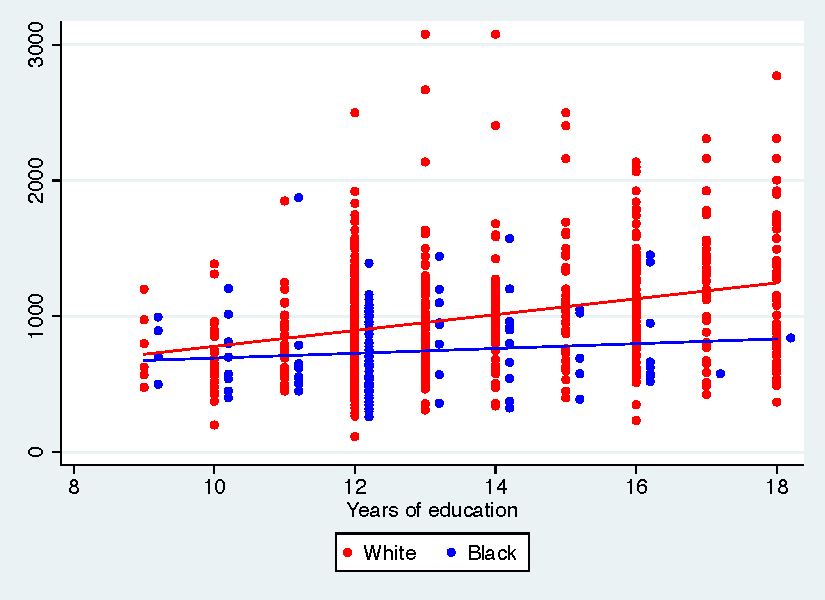
\includegraphics{interact1}
\end{figure}


The specification of an
interaction between a binary variable and a continous variable would
look like this:


\begin{stlog}
     
. reg lwage hours age educ black i.black#c.educ married  iq meduc south urban

      Source |       SS       df       MS              Number of obs =     857
-------------+------------------------------           F( 10,   846) =   29.69
       Model |  38.7974052    10  3.87974052           Prob > F      =  0.0000
    Residual |  110.563646   846  .130689889           R-squared     =  0.2598
-------------+------------------------------           Adj R-squared =  0.2510
       Total |  149.361051   856  .174487209           Root MSE      =  .36151

------------------------------------------------------------------------------
       lwage |      Coef.   Std. Err.      t    P>|t|     [95% Conf. Interval]
-------------+----------------------------------------------------------------
       hours |  -.0063045     .00173    -3.64   0.000    -.0097001    -.002909
         age |   .0215072   .0040455     5.32   0.000     .0135669    .0294476
        educ |   .0378404   .0069883     5.41   0.000     .0241239    .0515569
       black |   .1034702   .2766783     0.37   0.709    -.4395862    .6465265
             |
black#c.educ |
          1  |  -.0196117   .0215854    -0.91   0.364    -.0619789    .0227554
             |
     married |   .2051596   .0402851     5.09   0.000     .1260892      .28423
          iq |   .0040191   .0010442     3.85   0.000     .0019695    .0060687
       meduc |   .0102747   .0047964     2.14   0.032     .0008604    .0196889
       south |   -.069586   .0276172    -2.52   0.012    -.1237922   -.0153798
       urban |    .179133   .0281112     6.37   0.000     .1239572    .2343088
       _cons |    5.05532    .187864    26.91   0.000     4.686586    5.424055
------------------------------------------------------------------------------

. 
\end{stlog}


\subsection{Quick Exercise}

Run a regression with an interaction between urban and
education. Interpret the results. 

\subsection{Interactions with two continous variables}
\label{sec:inter-with-two-1}

Finally let's say we think that eductation will affect your wages
differently depending on your age. The specification of an interaction
between two continous variables would look like this: 


\begin{stlog}
  
. reg lwage hours age educ c.age#c.educ black married iq meduc south urban 

      Source |       SS       df       MS              Number of obs =     857
-------------+------------------------------           F( 10,   846) =   30.08
       Model |  39.1769054    10  3.91769054           Prob > F      =  0.0000
    Residual |  110.184146   846  .130241307           R-squared     =  0.2623
-------------+------------------------------           Adj R-squared =  0.2536
       Total |  149.361051   856  .174487209           Root MSE      =  .36089

------------------------------------------------------------------------------
       lwage |      Coef.   Std. Err.      t    P>|t|     [95% Conf. Interval]
-------------+----------------------------------------------------------------
       hours |  -.0066151   .0017294    -3.83   0.000    -.0100095   -.0032208
         age |  -.0280105   .0260076    -1.08   0.282    -.0790575    .0230364
        educ |  -.0876756   .0645406    -1.36   0.175    -.2143541    .0390029
             |
c.age#c.educ |   .0037019   .0019136     1.93   0.053    -.0000542    .0074579
             |
       black |  -.1466181   .0430343    -3.41   0.001    -.2310847   -.0621515
     married |   .2063299   .0402134     5.13   0.000     .1274003    .2852596
          iq |   .0040003   .0010423     3.84   0.000     .0019545    .0060461
       meduc |   .0100804   .0047844     2.11   0.035     .0006897     .019471
       south |    -.06698   .0276104    -2.43   0.015     -.121173    -.012787
       urban |    .182844     .02813     6.50   0.000     .1276312    .2380569
       _cons |   6.747921   .8848456     7.63   0.000     5.011171    8.484672
------------------------------------------------------------------------------

. 
\end{stlog}

The do file has extensive examples of how to use margins to create
nice plots of various types of interactions. We'll go over these in class.

\section{Not-so-quick Exercise}
\label{sec:not-so-quick}

In pairs, I would like you to estimate the best possible model using
the wage2 dataset. Think about model specification and functional
form, with an eye toward possible non-linearities and other
issues. Generate a do file that walks through your process of
identifying the best model.  Generate a fancy graph that shows the
predictions made by your model. 

\end{document}
